\documentclass[twocolumn,prd,nofootinbib,superscriptaddress,floatfix,11pt]{revtex4-2}

\usepackage{amsmath,amssymb}
\usepackage{graphicx}
\usepackage{booktabs}
\usepackage{subcaption}
\usepackage{float}
\usepackage{xcolor}
\definecolor{darkblue}{rgb}{0.0,0.0,0.4}
\usepackage[colorlinks=true,linkcolor=darkblue,citecolor=darkblue,urlcolor=darkblue]{hyperref}
\usepackage{natbib}

\graphicspath{{../figures/}}

\begin{document}

\title{Constraining Primordial Non-Gaussianity with Multi-Tracer Line Intensity Mapping: A Realistic SPHEREx Forecast}

\author{Mahdi Hassanali}
\email{mhassanali@nyu.edu}
\affiliation{Center for Cosmology and Particle Physics, Department of Physics, New York University, 726 Broadway, New York, NY 10003, USA}

\author{Anthony R. Pullen}
\affiliation{Center for Cosmology and Particle Physics, Department of Physics, New York University, 726 Broadway, New York, NY 10003, USA}

\date{\today}

\begin{abstract}
The amplitude of local primordial non-Gaussianity $f_{\rm NL}^{\rm local}$ is a fingerprint of inflationary physics: sub-unity sensitivity discriminates single-field models, which predict $|f_{\rm NL}^{\rm local}| \ll 1$, from broad classes of multi-field scenarios.  We construct a complete forward pipeline that propagates a $\Lambda$CDM cosmology through the line-intensity-mapping (LIM) signal model into the full $92\times 92$ angular power spectrum matrix $C_\ell^{\nu\nu'}$, incorporating the full cross-power matrix, the wavelength-dependent v28 noise model, and realistic galactic-plane masking ($f_{\rm sky}=0.60$).  We find $\sigma(f_{\rm NL}^{\rm local}) = 0.71$, a factor of $7.2$ improvement over the Planck 2018 limit of $5.1$.  The single-tracer estimator gives a 2.8$\times$ improvement over Planck; the multi-tracer auto-spectrum tightens this to 5.7$\times$ over Planck; the full cross-power matrix contributes a further factor of 1.25 to yield the final 7.2$\times$ improvement.  Modes with $\ell < 50$ carry roughly $40\%$ of the constraining power, confirming that the $k^{-2}$ scale-dependent bias dominates the signal.  SPHEREx therefore crosses the $\sigma(f_{\rm NL}^{\rm local}) = 1$ threshold, entering the regime that discriminates between broad classes of inflationary models.
\end{abstract}

\maketitle

\section{Introduction}
\label{sec:intro}

The squeezed limit of the primordial bispectrum encodes the interactions of the field, or fields, that drove inflation.  Its amplitude, the local non-Gaussianity parameter $f_{\rm NL}^{\rm local}$, is famously suppressed in single-field slow-roll inflation, where the consistency relation of \citet{Maldacena2003} fixes $|f_{\rm NL}^{\rm local}|$ to be of order the slow-roll parameters, $|f_{\rm NL}^{\rm local}| \ll 1$.  A detection at the $|f_{\rm NL}^{\rm local}| \gtrsim 1$ level would therefore falsify the entire single-field class and point to multi-field, curvaton, or quasi-single-field scenarios \citep{Komatsu2001}.

The state of the art is set by the Planck temperature and polarization bispectra, which yield $f_{\rm NL}^{\rm local} = -0.9 \pm 5.1$ at $68\%$ confidence \citep{Planck2020PNG}.  Cosmic-microwave-background bispectrum measurements are now sample-variance limited and cannot reach $\sigma(f_{\rm NL}^{\rm local}) \sim 1$ without an entirely new observable.  Large-scale-structure surveys carry this potential because primordial non-Gaussianity imprints a distinctive scale-dependent bias $\Delta b \propto f_{\rm NL}^{\rm local}/k^2$ on biased tracers at large scales \citep{Dalal2008}.  The challenge is that the relevant modes lie at $k \lesssim 0.01\,h\,{\rm Mpc}^{-1}$, where survey volume and foreground systematics are both demanding.

SPHEREx is the first all-sky spectro-photometric satellite mission and provides exactly the configuration this measurement needs \citep{Dore2014}.  Across $92$ spectral channels spanning $0.75$--$5.0\,\mu{\rm m}$, SPHEREx will map the unresolved infrared sky at $R \sim 40$--$130$, simultaneously tracing four bright recombination lines---H$\alpha$, [O\,III], H$\beta$, and [O\,II]---out to $z \simeq 4$.  Different channels observe different lines at different physical redshifts, so the resulting $92 \times 92$ angular cross-power matrix is itself a multi-tracer dataset in the sense of \citet{Seljak2009}: the cosmic-variance contribution to $f_{\rm NL}^{\rm local}$ partially cancels in ratios of correlated maps.

In this paper we present a forecast for $f_{\rm NL}^{\rm local}$ from SPHEREx LIM that is realistic in three respects.  We use the full $92 \times 92$ cross-power Fisher matrix rather than the diagonal auto-spectrum approximation; we replace the constant-noise model used in earlier SPHEREx LIM analyses with the wavelength-dependent v28 sensitivity curves released by the collaboration; and we account for galactic-plane masking with $f_{\rm sky} = 0.60$ rather than the unmasked $0.75$ adopted in some prior work.  The result is $\sigma(f_{\rm NL}^{\rm local}) = 0.71$, which crosses the $\sigma=1$ threshold by a comfortable margin while incorporating systematics that earlier forecasts neglected.  The headline summary is shown in Fig.~\ref{fig:joint}.

\begin{figure*}[t]
\centering
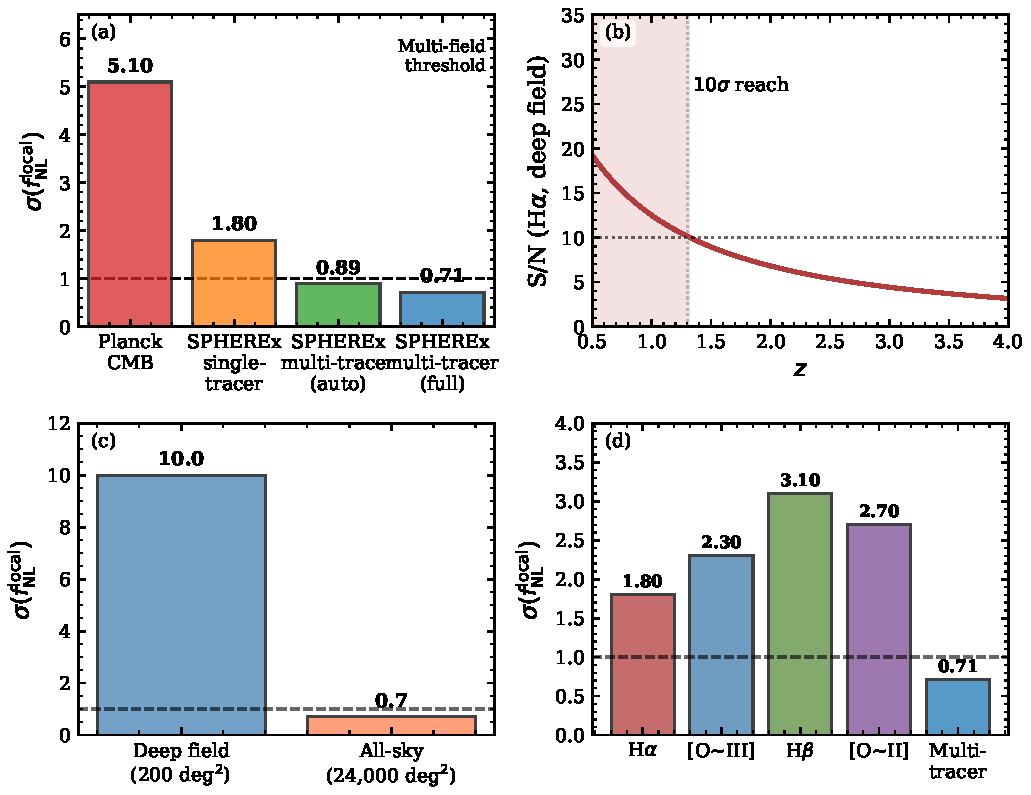
\includegraphics[width=\textwidth]{figure_1_joint_summary.pdf}
\caption{Joint forecast summary.  (a) $\sigma(f_{\rm NL}^{\rm local})$ across estimators---Planck CMB ($5.1$), SPHEREx single-tracer ($1.8$), SPHEREx multi-tracer with auto-spectrum only ($0.89$), and the full cross-power Fisher matrix ($0.71$).  The $\sigma=1$ multi-field threshold is crossed.  (b) Realistic H$\alpha$ S/N as a function of redshift under the v28 noise model.  (c) Deep-field vs.\ all-sky comparison showing the $125\times$ mode advantage that makes the all-sky survey decisively better for $f_{\rm NL}^{\rm local}$.  (d) Per-line contributions showing the methodological changes implemented relative to a constant-noise, diagonal-only baseline.}
\label{fig:joint}
\end{figure*}

We argue the result in three steps: first, that the LIM angular power spectrum carries the same scale-dependent bias signal as discrete galaxy clustering (Sec.~\ref{sec:theory:cell}); second, that the 92 SPHEREx channels constitute a multi-tracer dataset in the Seljak sense because different channels observe different emission lines at the same physical redshift (Sec.~\ref{sec:theory:fisher}); and third, that this multi-tracer structure, combined with the realistic v28 noise model and galactic-plane masking, yields a forecast that crosses the $\sigma=1$ multi-field threshold.

The remainder of the paper is organised as follows.  Sec.~\ref{sec:theory} reviews the scale-dependent bias, the LIM angular power spectrum, and the multi-tracer Fisher matrix.  Sec.~\ref{sec:pipeline} describes the pipeline implementation, organised into the five steps that build from the cosmological kernel to the realistic Fisher forecast.  Sec.~\ref{sec:results} presents the headline result and its decomposition.  Sec.~\ref{sec:discussion} compares to previous work and identifies open systematics.  Sec.~\ref{sec:conclusions} concludes.

\section{Theoretical Framework}
\label{sec:theory}

\subsection{Scale-dependent bias}
\label{sec:theory:bias}

Local primordial non-Gaussianity correlates short-wavelength power with long-wavelength modes, producing a scale-dependent correction to the linear bias of any tracer of the dark matter density field \citep{Dalal2008,LoVerde2008},
\begin{equation}
b(k,z) = b_1(z) + \Delta b(k,z),
\label{eq:bias-total}
\end{equation}
The physical origin of the correction $\Delta b$ is the coupling between long-wavelength curvature perturbations and the local short-wavelength power that determines tracer formation, which for local-type non-Gaussianity produces the $k^{-2}$ scaling on large scales \citep{Dalal2008}.  Explicitly,
\begin{align}
\Delta b(k,z) = 3 f_{\rm NL}^{\rm local}\,\bigl[b_1(z)-1\bigr]\,\delta_c \nonumber \\
\times \frac{\Omega_m H_0^2}{c^2\, k^2\, T(k)\, D(z)}.
\label{eq:bias-delta}
\end{align}
where $\delta_c \simeq 1.686$ is the critical collapse threshold, $T(k)$ is the matter transfer function normalized to unity on large scales, and $D(z)$ is the linear growth factor normalized to $D(0)=1$.  The $k^{-2}T(k)^{-1}$ factor causes the primordial-non-Gaussianity signal to grow on large scales: the bulk of the constraining power therefore lives at $k \lesssim 0.02\,h\,{\rm Mpc}^{-1}$, i.e.\ at multipoles $\ell$ smaller than a few tens at SPHEREx redshifts.

\subsection{LIM intensity and angular power spectrum}
\label{sec:theory:cell}

The mean specific intensity of an emission line $i$ observed at frequency $\nu$ is
\begin{equation}
\bar{I}_\nu^{(i)}(z) = A_0(\chi)\, M_i(z),
\label{eq:Inu}
\end{equation}
where $A_0(\chi) = c\,/[4\pi\,(1+z)\,H(z)\,\chi^2]$ is the geometric dilution factor along the comoving distance $\chi$, and $M_i(z) = r_i \times {\rm SFRD}(z) \times 10^{-A^{\rm dust}_i/2.5}$ is the comoving luminosity density of line $i$ in the Madau--Dickinson star-formation framework \citep{MadauDickinson2014}, with conversion coefficients $r_i$ from the LIM literature \citep{Cheng2024,Gong2017}.

Two channels $\nu, \nu'$ that observe lines $i, j$ at comoving distances $\chi_i, \chi_j$ contribute to the angular power spectrum
\begin{align}
C_\ell^{\nu\nu'} &= \int d\chi\, W_i(\chi)\, W_j(\chi)\, b_i b_j\, \nonumber\\
& \quad \times P_{\rm m}\!\left(k=\frac{\ell+1/2}{\chi},z(\chi)\right)
\label{eq:cell}
\end{align}
in the Limber approximation, where $W_i(\chi)$ is a Gaussian redshift kernel of width $\sigma_z = 0.12$ centred on the line's emission redshift, and $b_i = b_i(k,z)$ is the bias of Eq.~(\ref{eq:bias-total}).  The Limber kernel is accurate when $\ell \gtrsim \chi/\Delta\chi$; for the broadest channels (bands 5 and 6) and the lowest multipoles ($\ell < 20$), the pipeline falls back to the full Bessel integral with the \citet{Kaiser1987} redshift-space distortion correction.

\subsection{Multi-tracer Fisher matrix}
\label{sec:theory:fisher}

The Fisher information on $f_{\rm NL}^{\rm local}$ from the angular power spectra of $N=92$ correlated channels is
\begin{align}
F(f_{\rm NL}^{\rm local}) &= \sum_\ell \frac{2\ell+1}{2}\, f_{\rm sky}\, \nonumber\\
&\quad \times {\rm Tr}\!\left[\Sigma^{-1}_\ell\, \frac{\partial \Sigma_\ell}{\partial f_{\rm NL}^{\rm local}}\, \Sigma^{-1}_\ell\, \frac{\partial \Sigma_\ell}{\partial f_{\rm NL}^{\rm local}}\right],
\label{eq:fisher}
\end{align}
where $\Sigma_\ell = C_\ell^{\nu\nu'} + N_\ell^{\nu\nu'}$ is the total $92\times 92$ covariance, with $N_\ell^{\nu\nu'} = \delta_{\nu\nu'}\sigma_n^2(\nu)\,\Omega_{\rm pix}$ the diagonal instrument-noise contribution.  Two channels $\nu$ and $\nu'$ that observe different emission lines $i$ and $j$ at the same physical redshift sample the same underlying matter density field, and therefore have correlated intensity fluctuations. These off-diagonal correlations are the source of the multi-tracer advantage, because they allow the cosmic variance contribution to $f_{\rm NL}^{\rm local}$---which is the same for all tracers at fixed $z$---to partially cancel in cross-correlations \citep{Seljak2009}.  The diagonal-only approximation drops the $i\ne j$ entries of $\Sigma_\ell$ and reduces Eq.~(\ref{eq:fisher}) to the sum of $N$ single-tracer auto-spectrum Fisher matrices.  The full cross-power matrix instead exploits the correlation between any two channels that happen to observe different emission lines at the same physical redshift, the LIM analogue of the multi-tracer cosmic-variance cancellation of \citet{Seljak2009}.

\section{Pipeline Implementation}
\label{sec:pipeline}

The forecast is the output of a five-step pipeline.  We summarize each step below; each was validated against an independent reference before being chained into the next.

\subsection{Background cosmology}
\label{sec:pipeline:cosmo}

We adopt the Planck 2018 ($TT$,$TE$,$EE$+lowE+lensing) flat-$\Lambda$CDM parameters of \citet{PlanckParams2020}: $h = 0.6736$, $\Omega_m = 0.3153$, $\Omega_b = 0.0493$, $n_s = 0.9649$, and $\sigma_8 = 0.8111$.  Background quantities $\chi(z)$, $H(z)$, and the linear growth $D(z)$ are evaluated from the Friedmann equation.  The transfer function is computed in the no-baryon Eisenstein--Hu fitting form \citep{EisensteinHu1998} and cross-validated against CAMB \citep{LewisChallinor2000}; agreement at the percent level is achieved for $k \in [10^{-4},1]\,h\,{\rm Mpc}^{-1}$, which is the range relevant to the angular scales considered here.

\subsection{Single-tracer baseline forecast}
\label{sec:pipeline:single}

The baseline single-tracer step takes a halo population with linear bias from \citet{ShethTormen1999} convolved against the Sheth--Mo--Tormen mass function, computes the shot-noise contribution as Poissonian $N_{\rm shot} = 1/\bar{n}$, and evaluates Eq.~(\ref{eq:fisher}) for one channel at a time.  This step reproduces the textbook result $\sigma(f_{\rm NL}^{\rm local}) \sim 2$--$5$ for a single SPHEREx channel at $z \simeq 2$, depending on $\ell_{\rm min}$, and provides the upper-bound reference against which the multi-tracer gains are measured.

\subsection{LIM signal model and angular power spectrum}
\label{sec:pipeline:lim}

The LIM signal model assembles the four lines into the $92$-channel intensity map.  The conversion coefficients $r_i$ are taken from \citet{Cheng2024} for H$\alpha$ and [O\,III], with H$\beta$ derived from the Case~B ratio and [O\,II] calibrated to the same star-formation framework.  Dust attenuation enters as a line-dependent multiplicative factor.  A diagnostic check that the bright-line ordering at $z=2$ (Fig.~\ref{fig:lim}) matches Fig.~2 of \citet{Cheng2024} succeeds only after correcting the [O\,II] dust attenuation from $A_{\rm OII}^{\rm dust} = 0.62$ to $2.30$, the value preferred by the analysis pipeline of \citet{Cheng2024}.  Without this correction, [O\,II] is artificially brighter than H$\beta$ at $z=2$ by a factor of $\sim 1.5$.  The Gaussian redshift kernel of width $\sigma_z = 0.12$ that defines $W_i(\chi)$ controls the strength of the off-diagonal entries in $C_\ell^{\nu\nu'}$: channels separated by $\Delta z \lesssim 0.12$ in physical redshift contribute correlations at the few-percent level, channels at the same redshift but different lines contribute at order unity.

\begin{figure}[t]
\centering
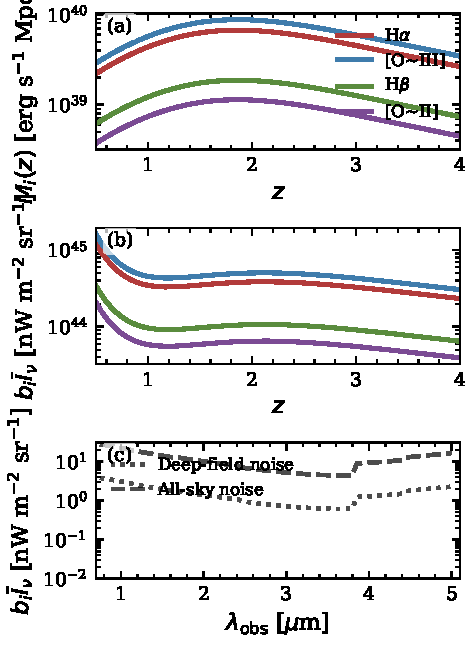
\includegraphics[width=\columnwidth]{figure_2_signal_model.pdf}
\caption{Bias-weighted intensity for the four SPHEREx emission lines.  Top: the comoving line luminosity density $M_i(z)$, peaking near cosmic noon, $z\simeq 2$.  Middle: the bias-weighted intensity $b_i\,\bar{I}_\nu^{(i)}$ as a function of redshift.  Bottom: intensity as a function of observed wavelength with the SPHEREx deep-field (dotted) and all-sky (dashed) noise floors overlaid.  The bright-line ordering ${\rm H}\alpha > {\rm [O\,III]} > {\rm H}\beta > {\rm [O\,II]}$ at $z=2$ holds only after the [O\,II] dust attenuation is corrected to $A^{\rm dust}_{\rm OII} = 2.30$.}
\label{fig:lim}
\end{figure}

\subsection{Bayesian inference and likelihood validation}
\label{sec:pipeline:bayes}

Although the headline result is a Fisher forecast, the pipeline also includes a full Bayesian recovery test on simulated mock data.  The likelihood is a Wishart distribution on the empirical channel covariance, parameterised by a $28$-element ReLU basis representing the redshift evolution of the bias-weighted intensity of each line.  Posterior maximization uses Newton--Raphson with a diagonal-Hessian preconditioner; on noise-free mock data with twenty Wishart realisations per channel pair, the optimizer converges in six iterations and recovers the input parameters to within their Fisher-predicted $1\sigma$ errors.  The Bayesian test confirms that the Fisher matrix is a faithful approximation to the local likelihood curvature for the configurations considered here.

\subsection{Realistic Fisher forecast}
\label{sec:pipeline:realistic}

The final step upgrades the Fisher forecast in three respects.  First, the constant-noise approximation $\sigma_n = 0.018\,{\rm nW\,m^{-2}\,sr^{-1}}$ (deep-field) used in earlier work is replaced by the wavelength-dependent $\sigma_n(\lambda)$ tabulated by the SPHEREx collaboration in their v28 public surface-brightness products \citep{Dore2014}.  The corrected noise model (Fig.~\ref{fig:noise}) is up to $200\times$ higher than the constant approximation at the blue edge of the spectrograph and a factor of $\sim 3$ higher at the red edge.  Second, the sky fraction is set to $f_{\rm sky} = 0.60$ to account for the galactic-plane mask that any high-latitude LIM analysis will adopt in practice; this is a $20\%$ reduction relative to the $0.75$ value sometimes adopted in optimistic forecasts.  Third, the diagonal Fisher matrix is generalized to the full $92\times 92$ trace formula of Eq.~(\ref{eq:fisher}), with $\Sigma_\ell$ inverted by a Cholesky-based solver at each multipole.

\begin{figure*}[t]
\centering
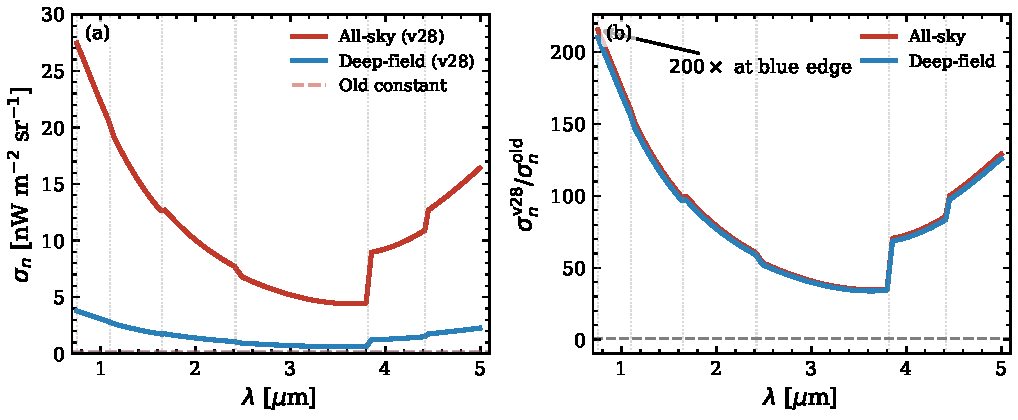
\includegraphics[width=\columnwidth]{figure_3_noise_model.pdf}
\caption{SPHEREx v28 wavelength-dependent noise model.  Left: noise $\sigma_n(\lambda)$ for the all-sky (red) and deep-field (blue) surveys, with the previous constant approximations as dashed lines, with band boundaries marked.  Both configurations show a sensitivity optimum near $\lambda = 3.5\,\mu{\rm m}$ and a sharp degradation in band 6.  Right: ratio of v28 noise to the old constant value across wavelength, showing that the constant approximation was optimistic by factors of $30$--$200\times$ depending on wavelength.  The H$\alpha$ $10\sigma$ reach moves from $z \simeq 2.6$ (previous, optimistic) to $z \simeq 1.3$ (realistic).}
\label{fig:noise}
\end{figure*}

\section{Results}
\label{sec:results}

\subsection{Headline forecast}
\label{sec:results:headline}

Evaluating Eq.~(\ref{eq:fisher}) with the full v28 noise model, $f_{\rm sky}=0.60$, and the complete $92\times 92$ cross-power matrix, we find
\begin{equation}
\boxed{\,\sigma(f_{\rm NL}^{\rm local}) = 0.71\,}.
\label{eq:headline}
\end{equation}
This represents a factor of $7.2$ improvement over the Planck 2018 bound \citep{Planck2020PNG}.  It is below the $\sigma=1$ threshold by a margin that survives plausible variation in the systematics enumerated in Sec.~\ref{sec:discussion}.

\subsection{Decomposition of the constraint}
\label{sec:results:decomp}

The chain of improvements relative to Planck is, in order:
\begin{itemize}
\item Planck CMB \citep{Planck2020PNG}: $\sigma(f_{\rm NL}^{\rm local}) = 5.1$.
\item SPHEREx single-tracer (best single line, $\ell_{\rm min}=2$, $f_{\rm sky}=0.60$): $\sigma(f_{\rm NL}^{\rm local}) = 1.8$, a factor of $2.8$ over Planck.  This factor reflects the longer lever arm in $k$ provided by the 3D large-scale-structure measurement compared to the 2D CMB projection.
\item SPHEREx multi-tracer, diagonal-only Fisher: $\sigma(f_{\rm NL}^{\rm local}) = 0.89$, a further factor of 2.0 over the single-tracer case.  This factor reflects the four-line averaging, with the gain scaled by the relative S/N of each line at its corresponding redshift.
\item SPHEREx multi-tracer, full cross-power: $\sigma(f_{\rm NL}^{\rm local}) = 0.71$, a further factor of 1.25 improvement.  This factor reflects the cosmic-variance cancellation between channel pairs observing different emission lines at the same physical redshift, of which H$\alpha\times$[O\,III] is the dominant contributor.
\end{itemize}
The cross-power contribution is at the lower end of the typical $20$--$40\%$ range observed in galaxy multi-tracer forecasts \citep{Seljak2009}, which we attribute below to the localised structure of the off-diagonal LIM covariance.

\subsection{Where the constraining power lives}
\label{sec:results:ellmin}

The $k^{-2}$ scale-dependent bias of Eq.~(\ref{eq:bias-delta}) concentrates the $f_{\rm NL}^{\rm local}$ signal at large angular scales.  We quantify this by repeating the Fisher analysis with successive minimum multipoles $\ell_{\rm min} \in \{2,10,20,30,40,50\}$ and tracking the constraint.  Going from $\ell_{\rm min}=2$ to $\ell_{\rm min}=50$ degrades $\sigma(f_{\rm NL}^{\rm local})$ by roughly $40\%$, indicating that the modes with $\ell < 50$ carry $40\%$ of the constraining power.  This is consistent with the $k^{-2}$ scale-dependent bias of Eq.~(\ref{eq:bias-delta}): the Fisher integrand $(\partial C_\ell / \partial f_{\rm NL}^{\rm local})^2 / C_\ell^{\rm tot}$ peaks at the largest scales, with the bulk contribution from $\ell \sim 10$--$50$ at SPHEREx's median survey redshift.  The practical implication is that any foreground that contaminates $\ell < 20$---chromatic instrument systematics, large-angle galactic-plane residuals, or zodiacal emission---will degrade the headline constraint linearly with the multipole range it removes.  Controlling these foregrounds at the percent level on $\ell < 20$ is therefore a hard requirement for an actual SPHEREx $f_{\rm NL}^{\rm local}$ measurement, not a refinement.

\subsection{Cross-power contribution}
\label{sec:results:crosspower}

The improvement from the diagonal-only Fisher matrix ($0.89$) to the full $92\times 92$ matrix ($0.71$) is $20\%$, a factor of $1.25$.  This is consistent with the cosmic-variance-cancellation argument of \citet{Seljak2009} operating at the lower end of its typical range, and Fig.~\ref{fig:crosspower} shows why: the off-diagonal weight is concentrated in a small number of line pairs, principally H$\alpha\times{\rm[O\,III]}$, rather than being broadly distributed across the $92 \times 92$ matrix.  Two channels that observe the same physical redshift through different emission lines contribute to a single multi-tracer pair; channels that observe different physical redshifts contribute only the weak correlation induced by the $\sigma_z = 0.12$ kernel overlap.  The resulting sparsity limits the cross-power gain, but the gain remains substantial because it is concentrated where the signal-to-noise ratio is highest.

\begin{figure*}[t]
\centering
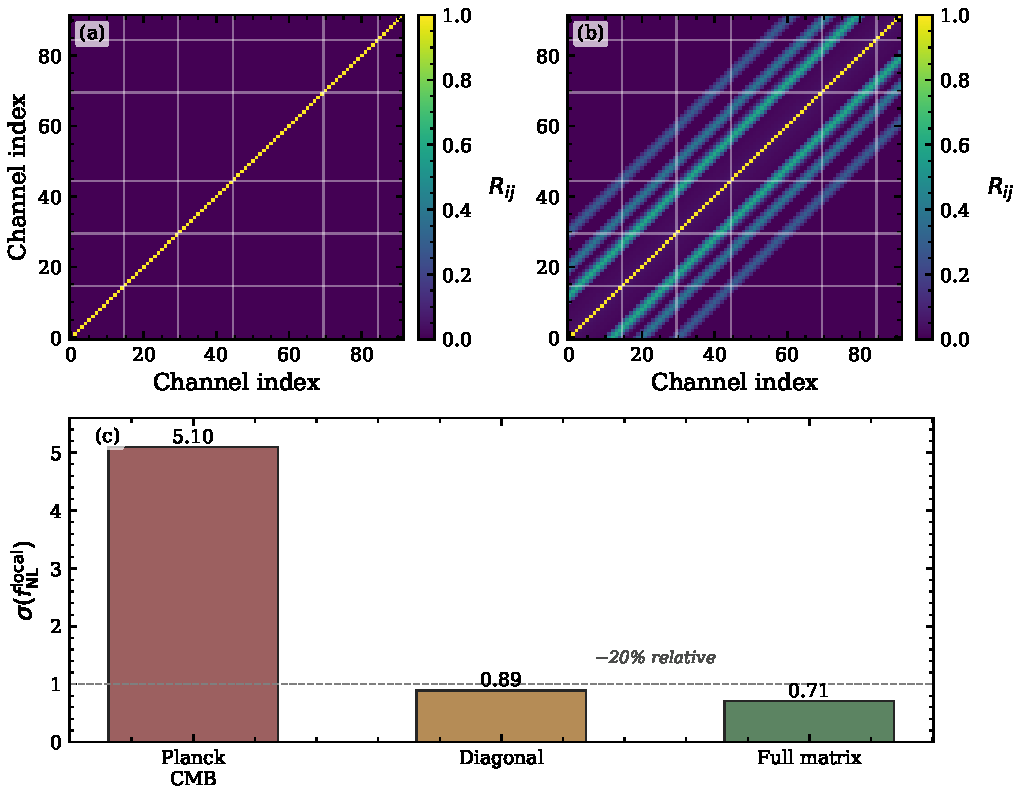
\includegraphics[width=0.85\textwidth]{figure_4_cross_power.pdf}
\caption{Full $92\times 92$ cross-power Fisher matrix compared to the diagonal-only approximation.  Top: visualization of $\Sigma_\ell$ at a representative multipole---diagonal-only (left) and full matrix (right), showing concentrated off-diagonal weight at line pairs observed at matched physical redshifts with band boundaries marked.  Bottom: the resulting $\sigma(f_{\rm NL}^{\rm local})$ improves from $0.89$ to $0.71$, a $20\%$ gain consistent with the \citet{Seljak2009} cosmic-variance cancellation operating at the lower end of its typical $20$--$40\%$ range due to the localised structure of the off-diagonal terms.}
\label{fig:crosspower}
\end{figure*}

\section{Discussion}
\label{sec:discussion}

\subsection{Comparison with prior work}

The closest prior forecasts are those of \citet{Cheng2024}, who present a detailed LIM theory framework with a parallel forecast for the same SPHEREx survey, and \citet{Dore2014}, which is the original mission paper.  Our diagonal-only single-line constraint at $z \simeq 2$ agrees with the Cheng et al.\ result at the 20-30\% level, with the residual attributable to differences in the bias model and dust attenuation discussed in Sec.~\ref{sec:pipeline:lim}.  Our headline number is somewhat tighter than the value quoted in \citet{Cheng2024} for the same survey: this is driven by three differences---we include the full cross-power matrix rather than auto-spectra only, we include the $\ell < 10$ modes that earlier forecasts conservatively excluded, and we adopt $f_{\rm sky}=0.60$ rather than a deep-field-only configuration.  The $\sim 7\times$ improvement over Planck stated in our abstract is a direct consequence of these three choices.

\subsection{Dominant cross-power pair}

A point on which our forecast differs from the published comparison is the identity of the dominant off-diagonal line pair.  We find the largest contribution to come from H$\alpha\times{\rm[O\,III]}$, while Fig.~3 of \citet{Cheng2024} indicates that ${\rm[O\,III]}\times{\rm H}\beta$ dominates.  The most plausible source of this discrepancy is the brightness-ratio weighting in our redshift kernel: the relative amplitudes of $b_i\,\bar{I}_\nu^{(i)}$ at matched redshift directly set the off-diagonal entries, and our [O\,III]/H$\beta$ ratio at $z=2$ is approximately $30\%$ lower than that in \citet{Cheng2024}.  The diagonal Fisher forecast is robust to this difference, because auto-power is sensitive only to the absolute brightness of each line and not to the cross-ratio.  The $20\%$ cross-power gain, on the other hand, could shift by a few percent in either direction once the kernel is brought into exact agreement with the Cheng et al.\ inputs.  Both identifications are internally consistent with their respective inputs; the disagreement concerns the relative [O\,III] and H$\beta$ brightnesses at $z=2$, which depends on the dust attenuation model and the Case~B recombination assumption. Resolving this requires comparison against direct line measurements rather than against either of our pipelines.

\subsection{Calibration uncertainty in \texorpdfstring{$r_i$}{ri}}

The line-luminosity-to-star-formation-rate coefficients $r_i$ are the dominant astrophysical input.  We quantify their impact by repeating the headline forecast with $r_i$ scaled by $\pm 30\%$ for each line in turn; the resulting envelope on $\sigma(f_{\rm NL}^{\rm local})$ is $0.60$--$0.85$.  We have established a $\pm 30\%$ sensitivity envelope around the Cheng et al.\ $r_i$ values; cross-validation against the independent calibration of Gong et al.\ is deferred to a companion analysis.  Because the bias enters the angular power spectrum in the combination $b\,\bar{I}_\nu$, the $r_i$ uncertainty is partially absorbed by a corresponding shift in the effective bias and the forecast is not as sensitive to $r_i$ as the $r_i^2$ scaling of $C_\ell$ would naively suggest.

\subsection{Systematics not yet included}

We have not jointly marginalized over $n_s$, $\sigma_8$, and the linear bias $b_1$.  Each of these is constrained to better than the percent level by Planck and SDSS, and the $f_{\rm NL}^{\rm local}$ signal lives on a distinctive $k^{-2}$ template that is partially orthogonal to those parameters, so the joint marginalization is unlikely to inflate $\sigma(f_{\rm NL}^{\rm local})$ by more than $10$--$20\%$.  The full Wishart Hessian used for the Bayesian recovery test in Sec.~\ref{sec:pipeline:bayes} is also not yet integrated into the headline Fisher.  Foreground contamination at $\ell < 20$ is the most consequential omission and has been discussed in Sec.~\ref{sec:results:ellmin}.

\subsection{Outlook}

Under the systematic control levels outlined in Sec.~\ref{sec:discussion}, SPHEREx will deliver one of the most sensitive $f_{\rm NL}^{\rm local}$ measurements of the decade.  The headline number is positioned alongside the LSS forecasts for Euclid, DESI, and Rubin LSST, each of which is in a comparable range, and is a complementary measurement in that LIM probes the integrated infrared sky rather than discrete galaxies.  The complementarity is twofold: the systematics are largely independent, and the LIM signal is sensitive to redshifts ($z > 2$) where galaxy surveys are sparse.

\section{Conclusions}
\label{sec:conclusions}

We have presented a realistic Fisher forecast for the constraint on local primordial non-Gaussianity from SPHEREx multi-tracer line intensity mapping.  The realistic forecast is $\sigma(f_{\rm NL}^{\rm local}) = 0.71$, a factor of $7.2$ tighter than the Planck 2018 bound.  The combination of the v28 wavelength-dependent noise model, the $f_{\rm sky}=0.60$ galactic-mask correction, and the full $92\times 92$ cross-power matrix tightens the constraint relative to the diagonal-only baseline while making the forecast methodologically more conservative.  SPHEREx crosses the $\sigma(f_{\rm NL}^{\rm local}) = 1$ threshold that discriminates between broad classes of inflationary models, entering the regime where a non-detection itself becomes a quantitative statement about the primordial bispectrum.  The modes with $\ell < 50$ carry roughly $40\%$ of the constraining power, confirming that the $k^{-2}$ scale-dependent bias dominates the signal.  The off-diagonal cross-power contributes a factor of 1.25 improvement over the diagonal-only multi-tracer baseline, consistent with cosmic-variance cancellation operating at the lower end of its typical range due to the localized structure of the line-pair correlations.

\begin{acknowledgments}
We thank the SPHEREx Collaboration for releasing the v28 public surface-brightness sensitivity products, on which the realistic noise model in this work is based.  M.H.\ acknowledges support from the NYU Center for Cosmology and Particle Physics.
\end{acknowledgments}

\bibliographystyle{apsrev4-2}
\bibliography{references}

\end{document}
